\documentclass[11pt,a4paper]{article}

\usepackage[T1]{fontenc}
\usepackage[utf8]{inputenc}
\usepackage{lmodern}
\usepackage[spanish,es-nodecimaldot]{babel}
\usepackage[margin=1.0in]{geometry}
\usepackage{amsmath,amssymb,amsfonts}
\usepackage{graphicx}
\usepackage{xcolor}
\usepackage{colortbl}
\usepackage{booktabs}
\usepackage{float}
\usepackage{hyperref}
\usepackage{tikz}
\usepackage{pgfplots}
\pgfplotsset{compat=1.16}
\usetikzlibrary{arrows.meta, shapes.geometric, fit, positioning, backgrounds}

\hypersetup{
    colorlinks=true,
    linkcolor=blue,
    urlcolor=blue,
    citecolor=blue
}

\title{\textbf{Hierarchical RDO-Trained Transform for Attribute-Dependent Point Cloud Compression}}
\author{\textbf{Simón Yáñez} \\ Information Decision Systems Group}
\date{}

\begin{document}

\maketitle

\begin{abstract}
La compresión eficiente de atributos de color (YUV) en nubes de puntos 3D densas requiere transformadas espectrales que se adapten a las discontinuidades y gradientes locales de la superficie sin sobrecargar el flujo binario con información de control. Este trabajo presenta un marco de Transformada de Fourier sobre Grafos (GFT) adaptativa con señalización desacoplada jerárquicamente. La metodología se estructura en tres etapas secuenciales: en primer lugar, la geometría se particiona en bloques macro padre y sub-bloques finos; en segundo lugar, se aprende un codebook estático fuera de línea mediante agrupamiento esférico sobre la variedad $\mathbb{S}^2$, calibrando la matriz de adyacencia y pesos de self-loop mediante optimización continua unidimensional para minimizar directamente el costo lagrangiano Rate-Distortion; finalmente, la señalización de modos se realiza exclusivamente a nivel macro mediante codificación aritmética contextual de primer orden (CABAC), mientras que los sub-bloques ejecutan transformadas direccionales de grano fino. Las evaluaciones empíricas sobre 14 secuencias (8iVFB y MVUB, profundidades 9 y 10) demuestran que el esquema propuesto logra una reducción física de BD-Rate promedio de \textbf{-2.03\%} (rango -1.14\% a -3.33\% según la secuencia, mejor configuración por secuencia) frente a la línea base estructural, con la ganancia agregada más alta en $B_c=16$ ($-1.98\% \pm 0.71$ en $K=24$, promedio y desviación estándar sobre las 14 secuencias). El decodificador autónomo reconstruye fielmente los atributos a partir únicamente de la geometría transmitida y el codebook pre-entrenado.
\end{abstract}

%==========================================================================
\section{Metodología Algorítmica Secuencial}
%==========================================================================

El esquema propuesto aborda la compresión de atributos mediante una secuencia algorítmica estructurada que desacopla la escala de decisión de la escala de transformación. A continuación se detalla el flujo de procesamiento paso a paso.

\subsection{Particionamiento Espacial Jerárquico}
La nube de puntos original, descrita por sus coordenadas geométricas $\mathbf{V} \in \mathbb{R}^{N_{\text{vox}} \times 3}$ y señales de luminancia $A_Y \in \mathbb{R}^{N_{\text{vox}}}$, se organiza mediante una curva espacial de Morton (orden z-order). 

El espacio volumétrico se particiona en dos niveles:
\begin{itemize}
  \item \textbf{Bloques Macro Padre ($B_p = 32$):} Bloques volumétricos de mayor tamaño ($N_p = 834$) donde se extrae la orientación geométrica dominante y se toma la decisión de modo.
  \item \textbf{Sub-bloques Hijos ($B_c \in \{32, 16, 8, 4\}$):} Particiones espaciales de granularidad fina sobre las cuales se construye el grafo local y se calcula la transformada espectral directa e inversa.
\end{itemize}

\subsection{Construcción de Grafos y Lógica de Nodos Sumidero (Sink Nodes)}
Para cada partición, la conectividad se define mediante un grafo no dirigido ponderado con conectividad de 26 vecinos. Los pesos geométricos estructurales se calculan como:
\begin{equation}
  W_{\text{str},ij} = 
  \begin{cases}
    \frac{1}{D_{ij}} & \text{si } 0 < D_{ij} \le \sqrt{3} + \epsilon \\[6pt]
    0 & \text{en otro caso},
  \end{cases}
\end{equation}
donde $D_{ij} = \|\mathbf{v}_i - \mathbf{v}_j\|_2$ es la distancia euclidiana entre vóxeles. La matriz de adyacencia se simetriza como $W_{\text{sym}} = W_{\text{str}} + W_{\text{str}}^T$.

Para incorporar direccionalidad dependiente del atributo, se proyecta un gradiente de señal sobre la superficie, generando una aproximación de luminancia $Y_{\text{approx}}$. La diferencia de señal entre nodos conectados define la matriz de flujo:
\begin{equation}
  M_{ij} = W_{\text{str},ij} \cdot (Y_{\text{approx},i} - Y_{\text{approx},j}).
\end{equation}

Cada nodo $i$ dirige su flujo hacia el vecino con mayor gradiente descendente. Aquellos nodos $j$ que reciben la mayor convergencia de flujo se denominan \textbf{nodos sumidero (sink nodes)}. La intensidad de sumidero se cuantifica como:
\begin{equation}
  S_j = \sum_{i} \mathbb{I}\left[\arg\min_m M_{im} = j\right].
\end{equation}

Para regular la señal en las fronteras y compactar la energía espectral en bajas frecuencias, una fracción $s_{\text{lp}}$ de los nodos con mayor valor $S_j$ recibe un peso de auto-bucle (\textbf{self-loop}) en la diagonal:
\begin{equation}
  W_{jj}^{\text{self}} = s_{\text{lw}}.
\end{equation}

La matriz Laplaciana direccional resultante se formula como:
\begin{equation}
  \mathbf{L}_{\text{attr}} = \mathbf{D}_{\text{attr}} - W_{\text{sym}} + \mathrm{diag}(W^{\text{self}}),
\end{equation}
donde $\mathbf{D}_{\text{attr}}$ es la matriz diagonal de grados. La base ortonormal de la GFT, $\mathbf{U}$, se obtiene resolviendo el problema de autovalores:
\begin{equation}
  \mathbf{L}_{\text{attr}} \mathbf{U} = \mathbf{U} \mathbf{\Lambda}.
\end{equation}

\subsection{Entrenamiento de Centroides Geométricos en $\mathbb{S}^2$}
Para representar los gradientes locales mediante un conjunto finito de $K$ modos, se entrena un codebook estático de centroides directores $\{c_k\}_{k=1}^{K-1} \subset \mathbb{S}^2$ fuera de línea (offline):
\begin{enumerate}
  \item \textbf{Extracción de Planos Tangentes:} En cada bloque padre se calcula la matriz de covarianza de coordenadas centradas, obteniendo los ejes tangentes principales $v_1, v_2$ y la normal $v_3$.
  \item \textbf{Ajuste de Pendientes 2D:} Se proyectan las coordenadas centradas sobre la base tangente $\mathbf{X} = [V v_1, \; V v_2]$ y se ajusta analíticamente la señal centrada $\mathbf{Y}$:
  \begin{equation}
    \mathbf{s}_{\text{2D}} = (\mathbf{X}^T \mathbf{X})^{-1} \mathbf{X}^T \mathbf{Y}.
  \end{equation}
  \item \textbf{Reconstrucción del Vector 3D:} El gradiente 3D se reconstruye como $\mathbf{g} = s_1 v_1 + s_2 v_2$, normalizándose sobre la esfera unitaria $\hat{\mathbf{g}} = \mathbf{g} / \|\mathbf{g}\|_2 \in \mathbb{S}^2$.
  \item \textbf{Filtrado de Textura por Percentil:} Los bloques con baja energía de gradiente ($\|\mathbf{g}\|_2 < \text{p50}$) se excluyen del entrenamiento para evitar que zonas planas sesguen las direcciones.
  \item \textbf{Clustering Esférico ($K$-Means Esférico):} Dado que los vectores directores son unitarios y residen sobre la superficie de la esfera $\mathbb{S}^2$, se emplea $K$-Means Esférico maximizando la similitud coseno absoluta $|\hat{\mathbf{g}} \cdot c_k|$. Esto asegura que direcciones antipodales opuestas pero paralelas ($\mathbf{g}$ y $-\mathbf{g}$) compartan el mismo modo. La actualización promedia los vectores asignados a cada grupo:
  \begin{equation}
    c_k \leftarrow \frac{\sum_{i \in \mathcal{C}_k} \text{sign}(\hat{\mathbf{g}}^{(i)} \cdot c_k) \hat{\mathbf{g}}^{(i)}}{\left\|\sum_{i \in \mathcal{C}_k} \text{sign}(\hat{\mathbf{g}}^{(i)} \cdot c_k) \hat{\mathbf{g}}^{(i)}\right\|_2}.
  \end{equation}
\end{enumerate}

\subsection{Optimización Continua de Parámetros del Grafo ($s_{\text{lp}}, s_{\text{lw}}$)}
Los centroides $\{c_k\}$ determinan la orientación del plano. Para definir cuantitativamente la fracción de sumideros ($s_{\text{lp}}$) y el peso del auto-bucle ($s_{\text{lw}}$) que maximizan la concentración de energía espectral en la transformada, se optimizan ambos parámetros minimizando el costo lagrangiano Rate-Distortion:
\begin{equation}
  J_{\text{block}} = \lambda_0 \cdot Q^2 \cdot \|\hat{\mathbf{c}}_q\|_0 + \|\mathbf{c} - \hat{\mathbf{c}}_{\text{dq}}\|_2^2,
\end{equation}
donde $\hat{\mathbf{c}}_q = \text{round}(\mathbf{U}^T A / Q)$ son los coeficientes cuantizados y $\|\cdot\|_0$ mide el número de coeficientes no nulos.

Para no depender de derivadas analíticas complejas del espectro de la matriz Laplaciana, la optimización se realiza en dos etapas continuas:
\begin{enumerate}
  \item \textbf{Búsqueda en Malla Inicial:} Se evalúa un conjunto discreto de candidatos $s_{\text{lp}} \in [0.05, 0.60]$ y $s_{\text{lw}} \in [0.15, 0.75]$ para localizar la región donde el costo lagrangiano es mínimo.
  \item \textbf{Refinamiento Continuo por Contracción de Intervalo:} Fijando el mejor $s_{\text{lp}}^*$, se aplica una búsqueda unidimensional continua que reduce iterativamente el rango de búsqueda evaluando puntos interiores en una proporción de $0.618$ (búsqueda por razón áurea). En sólo 4 evaluaciones, este método converge al peso de auto-bucle óptimo continuo $s_{\text{lw}}^* \in [0.05, 1.0]$:
  \begin{equation}
    (s_{\text{lp}}^*, s_{\text{lw}}^*) = \arg\min_{(p, w)} \sum_{b \in \text{SampleBlocks}} J_{\text{block}}\Big(\mathbf{U}_{k,(p,w)}^T A_b, \; Q\Big).
  \end{equation}
\end{enumerate}

\subsection{Desacoplamiento Jerárquico y Codificación Aritmética de Modos}
Para que la información de control no penalice a los sub-bloques pequeños, el sistema desacopla totalmente la decisión:
\begin{enumerate}
  \item \textbf{Optimización Global por Trellis de Viterbi:} La secuencia de modos $\{M_p\}_{p=1}^{N_p}$ para los bloques macro padre se selecciona minimizando el costo conjunto con penalización por cambios bruscos de dirección:
  \begin{equation}
    \min_{\{M_p\}} \sum_{p=1}^{N_p} J_{\text{parent},p}(M_p) + \gamma_0 \left(\frac{Q}{24}\right)^2 \sum_{p=2}^{N_p} |\mathbf{n}_p \cdot \mathbf{n}_{p-1}| \cdot \mathbb{I}[M_p \ne M_{p-1}].
  \end{equation}
  \item \textbf{Filtrado Causal (Causal Gating):} Si la varianza causal del bloque es baja ($\sigma^2(\hat{A}_Y) < \tau_{\text{gate}}$), el bloque se asigna automáticamente al Modo 0 (estructural) con \textbf{cero costo de señalización}.
  \item \textbf{Herencia Espacial en Sub-bloques:} Todos los sub-bloques hijos heredan directamente el modo $M_p$ del bloque macro padre que los contiene. Así, los miles de sub-bloques pequeños ejecutan la GFT direccional sin requerir bits de control adicionales.
\end{enumerate}

\subsection{Ejemplo de Estructuración y Decodificación del Overhead (CABAC)}
Para ilustrar con precisión qué codifica el encoder, cómo se construye el overhead y por qué su tamaño es tan bajo:
\begin{itemize}
  \item \textbf{Qué se codifica exactamente:} El encoder únicamente transmite la secuencia de índices de modo de los bloques macro padre activos, por ejemplo una secuencia de enteros $\{M_1, M_2, \dots, M_{N_{\text{active}}}\}$ donde cada $M_p \in \{1, 2, \dots, K-1\}$. Para una nube con 834 bloques macro padre, aproximadamente 780 son activos.
  \item \textbf{Cómo se comprime el overhead:} Dado que el recorrido sigue la curva espacial de Morton, bloques contiguos presentan orientaciones superficiales similares. Un codificador aritmético contextual (CABAC de primer orden) aprovecha esta correlación espacial modelando las probabilidades de transición condicionales $P(M_p \mid M_{p-1})$. 
  \item \textbf{Por qué el costo es mínimo:} En lugar de gastar bits por cada sub-bloque, sólo se codifican $\approx 780$ transiciones para todo el objeto 3D. Esto genera un archivo de sobrecarga de sólo $\approx 350\text{ bytes}$ en total. Dividido entre los $765{,}821$ vóxeles de la nube, la sobrecarga neta representa apenas:
  \begin{equation}
    \text{Overhead BPV} = \frac{350 \text{ Bytes} \times 8 \text{ bits/Byte}}{765{,}821 \text{ vóxeles}} \approx 0.0036 \text{ BPV}.
  \end{equation}
  \item \textbf{Cómo lo decodifica el receptor:} El decodificador lee la geometría $\mathbf{V}$, desempaqueta la secuencia de modos $\{M_p\}$ directamente desde el flujo CABAC y, para cada sub-bloque, consulta las coordenadas espaciales de su centro para heredar automáticamente el modo $M_p$ del bloque macro padre, reconstruyendo la base $\mathbf{U}_{M_p}$ a partir del codebook pre-entrenado sin requerir información adicional.
\end{itemize}

\begin{figure}[H]
\centering
\resizebox{\linewidth}{!}{%
\begin{tikzpicture}[
  node distance=0.50cm and 0.80cm,
  box/.style={draw, rounded corners=3pt, fill=blue!8, text width=3.2cm,
              align=center, font=\scriptsize, minimum height=0.75cm},
  proc/.style={draw, rounded corners=3pt, fill=green!10, text width=3.2cm,
              align=center, font=\scriptsize, minimum height=0.75cm},
  dec/.style={draw, diamond, fill=orange!15, text width=2.1cm,
              align=center, font=\scriptsize, aspect=1.8},
  bit/.style={draw, rounded corners=3pt, fill=purple!12, text width=3.2cm,
              align=center, font=\scriptsize, minimum height=0.75cm},
  cb/.style={draw=orange!80, fill=yellow!25, rounded corners=4pt, text width=2.8cm, align=center, font=\scriptsize, line width=1.1pt},
  arr/.style={-{Stealth[scale=0.85]}, thick},
  darr/.style={-{Stealth[scale=0.85]}, thick, dashed},
  grp/.style={draw=gray!50, rounded corners=6pt, dashed, inner sep=8pt}
]
  % ENCODER PIPELINE
  \node[box] (e_in) {Entrada: Geometría y Atributos\\$\mathbf{V}, \mathbf{A}$};
  \node[proc, below=of e_in] (e_part) {Particionado Jerárquico\\$B_p=32 \to B_c \in \{32,16,8,4\}$};
  \node[proc, below=of e_part] (e_pca) {Fase 1: Tangente PCA\\Spherical $K$-Means en $\mathbb{S}^2$};
  \node[proc, below=of e_pca] (e_rdo) {Fase 2: Optimización RDO\\Calibración $(s_{\text{lp}}, s_{\text{lw}})$};
  \node[proc, below=of e_rdo] (e_gft) {GFT Paralela en Sub-bloques\\$K$ Bases Espectrales $\mathbf{U}_k$};
  \node[dec, below=of e_gft] (e_gate) {Gating RDO\\$\sigma^2(A_Y) \ge \tau_{\text{gate}}$?};
  \node[box, below left=0.6cm and 0.1cm of e_gate] (e_m0) {Modo 0: Estructural\\(\textbf{0 bits señalización})};
  \node[proc, below right=0.6cm and 0.1cm of e_gate] (e_vit) {Trellis de Viterbi\\$\min \sum J + \gamma |v_3 \cdot v_3|$};
  \node[bit, below=1.8cm of e_gate] (e_bs) {Codificador PyRLGR + CABAC\\Bitstream $(\hat{\mathbf{c}}, M_p)$};

  \begin{scope}[on background layer]
    \node[grp, fit=(e_in)(e_part)(e_pca)(e_rdo)(e_gft)(e_gate)(e_m0)(e_vit)(e_bs), label=above:{\small\textbf{Pipeline del Codificador (Encoder)}}] {};
  \end{scope}

  \draw[arr] (e_in) -- (e_part);
  \draw[arr] (e_part) -- (e_pca);
  \draw[arr] (e_pca) -- (e_rdo);
  \draw[arr] (e_rdo) -- (e_gft);
  \draw[arr] (e_gft) -- (e_gate);
  \draw[arr] (e_gate) -- node[left,font=\tiny]{No} (e_m0);
  \draw[arr] (e_gate) -- node[right,font=\tiny]{Sí} (e_vit);
  \draw[arr] (e_m0) |- (e_bs);
  \draw[arr] (e_vit) |- (e_bs);

  % CENTRAL CHANNEL & OFFLINE CODEBOOK
  \node[bit, right=2.2cm of e_bs, fill=purple!20, text width=2.6cm] (channel) {\textbf{Canal / Bitstream}\\$\hat{\mathbf{c}}$ (PyRLGR)\\+ $M_p$ (CABAC)};
  \node[cb, above=4.5cm of channel] (codebook) {\textbf{Codebook Estático}\\Entrenado Offline\\$\{c_k\} \subset \mathbb{S}^2, (s_{\text{lp}}^*, s_{\text{lw}}^*)$};

  \draw[arr, ultra thick, color=purple!70] (e_bs) -- (channel);
  \draw[darr, color=gray!80] (codebook) -| (e_gft.north);

  % DECODER PIPELINE
  \node[bit, right=2.2cm of channel] (d_bs) {Descompresión Binaria\\PyRLGR ($\hat{\mathbf{c}}$) + CABAC ($M_p$)};
  \node[dec, above=1.8cm of d_bs] (d_check) {Modo $M_p = 0$?\\(Fallback/Gated)};
  \node[box, above left=0.6cm and 0.1cm of d_check] (d_m0) {iGFT Estructural\\(Sin Self-loops)};
  \node[proc, above right=0.6cm and 0.1cm of d_check] (d_parse) {iGFT Direccional\\Proyectar $c_{M_p}$ y $(s_{\text{lp}}, s_{\text{lw}})$};
  \node[proc, above=1.5cm of d_check] (d_igft) {Reconstrucción de Atributos\\$\hat{\mathbf{A}} = \mathbf{U}_{M_p} (Q \cdot \hat{\mathbf{c}})$};
  \node[proc, above=of d_igft] (d_oct) {Ensamblado de Sub-bloques\\Indexación Espacial};
  \node[box, above=of d_oct] (d_out) {Nube Reconstruida\\$\mathbf{V}, \hat{\mathbf{A}}$};

  \begin{scope}[on background layer]
    \node[grp, fit=(d_bs)(d_check)(d_m0)(d_parse)(d_igft)(d_oct)(d_out), label=above:{\small\textbf{Pipeline del Decodificador (Zero-Oracle Decoder)}}] {};
  \end{scope}

  \draw[arr, ultra thick, color=purple!70] (channel) -- (d_bs);
  \draw[arr] (d_bs) -- (d_check);
  \draw[arr] (d_check) -- node[left,font=\tiny]{Sí} (d_m0);
  \draw[arr] (d_check) -- node[right,font=\tiny]{No} (d_parse);
  \draw[arr] (d_m0) |- (d_igft);
  \draw[arr] (d_parse) |- (d_igft);
  \draw[arr] (d_igft) -- (d_oct);
  \draw[arr] (d_oct) -- (d_out);

  \draw[darr, color=gray!80] (codebook) -| (d_parse.north);
\end{tikzpicture}%
}
\caption{\textbf{Arquitectura Integral del Sistema:} Interacción asimétrica entre Codificador y Decodificador. En el codificador, el filtro $\tau_{\text{gate}}$ poda el espacio de búsqueda forzando modo 0 en zonas de baja varianza. El decodificador es puramente determinista y no requiere calcular varianzas: desempaqueta los índices de modo $M_p$ directamente desde el flujo CABAC y aplica la base ortonormal correspondiente.}
\label{fig:gating_pipeline}
\end{figure}

%==========================================================================
\section{Evaluación Experimental y Resultados de Tasa-Distorsión}
%==========================================================================

Las evaluaciones se realizan sobre 14 secuencias estándar: \texttt{longdress}, \texttt{loot}, \texttt{redandblack}, \texttt{soldier} (8iVFB, profundidad 10) y \texttt{andrew}, \texttt{david}, \texttt{phil}, \texttt{ricardo}, \texttt{sarah} (MVUB, profundidades 9 y 10), cubriendo las tasas de cuantización $Q \in \{24, 32, 48, 64\}$. Todas las comparaciones se realizan contra la línea base estructural estática emparejada con idéntico tamaño de bloque y cuantización $(B, Q)$. La escala $B_c=32$ (bloque hijo igual al bloque padre) permanece evaluada únicamente sobre \texttt{longdress} ($n=1$) por costo computacional (aproximadamente $15\times$ el tiempo de \texttt{longdress} en $B_c=16$ por combinación $(K,Q)$) y se reporta por separado, sin promediarla junto a las demás escalas.

\begin{figure}[H]
\centering
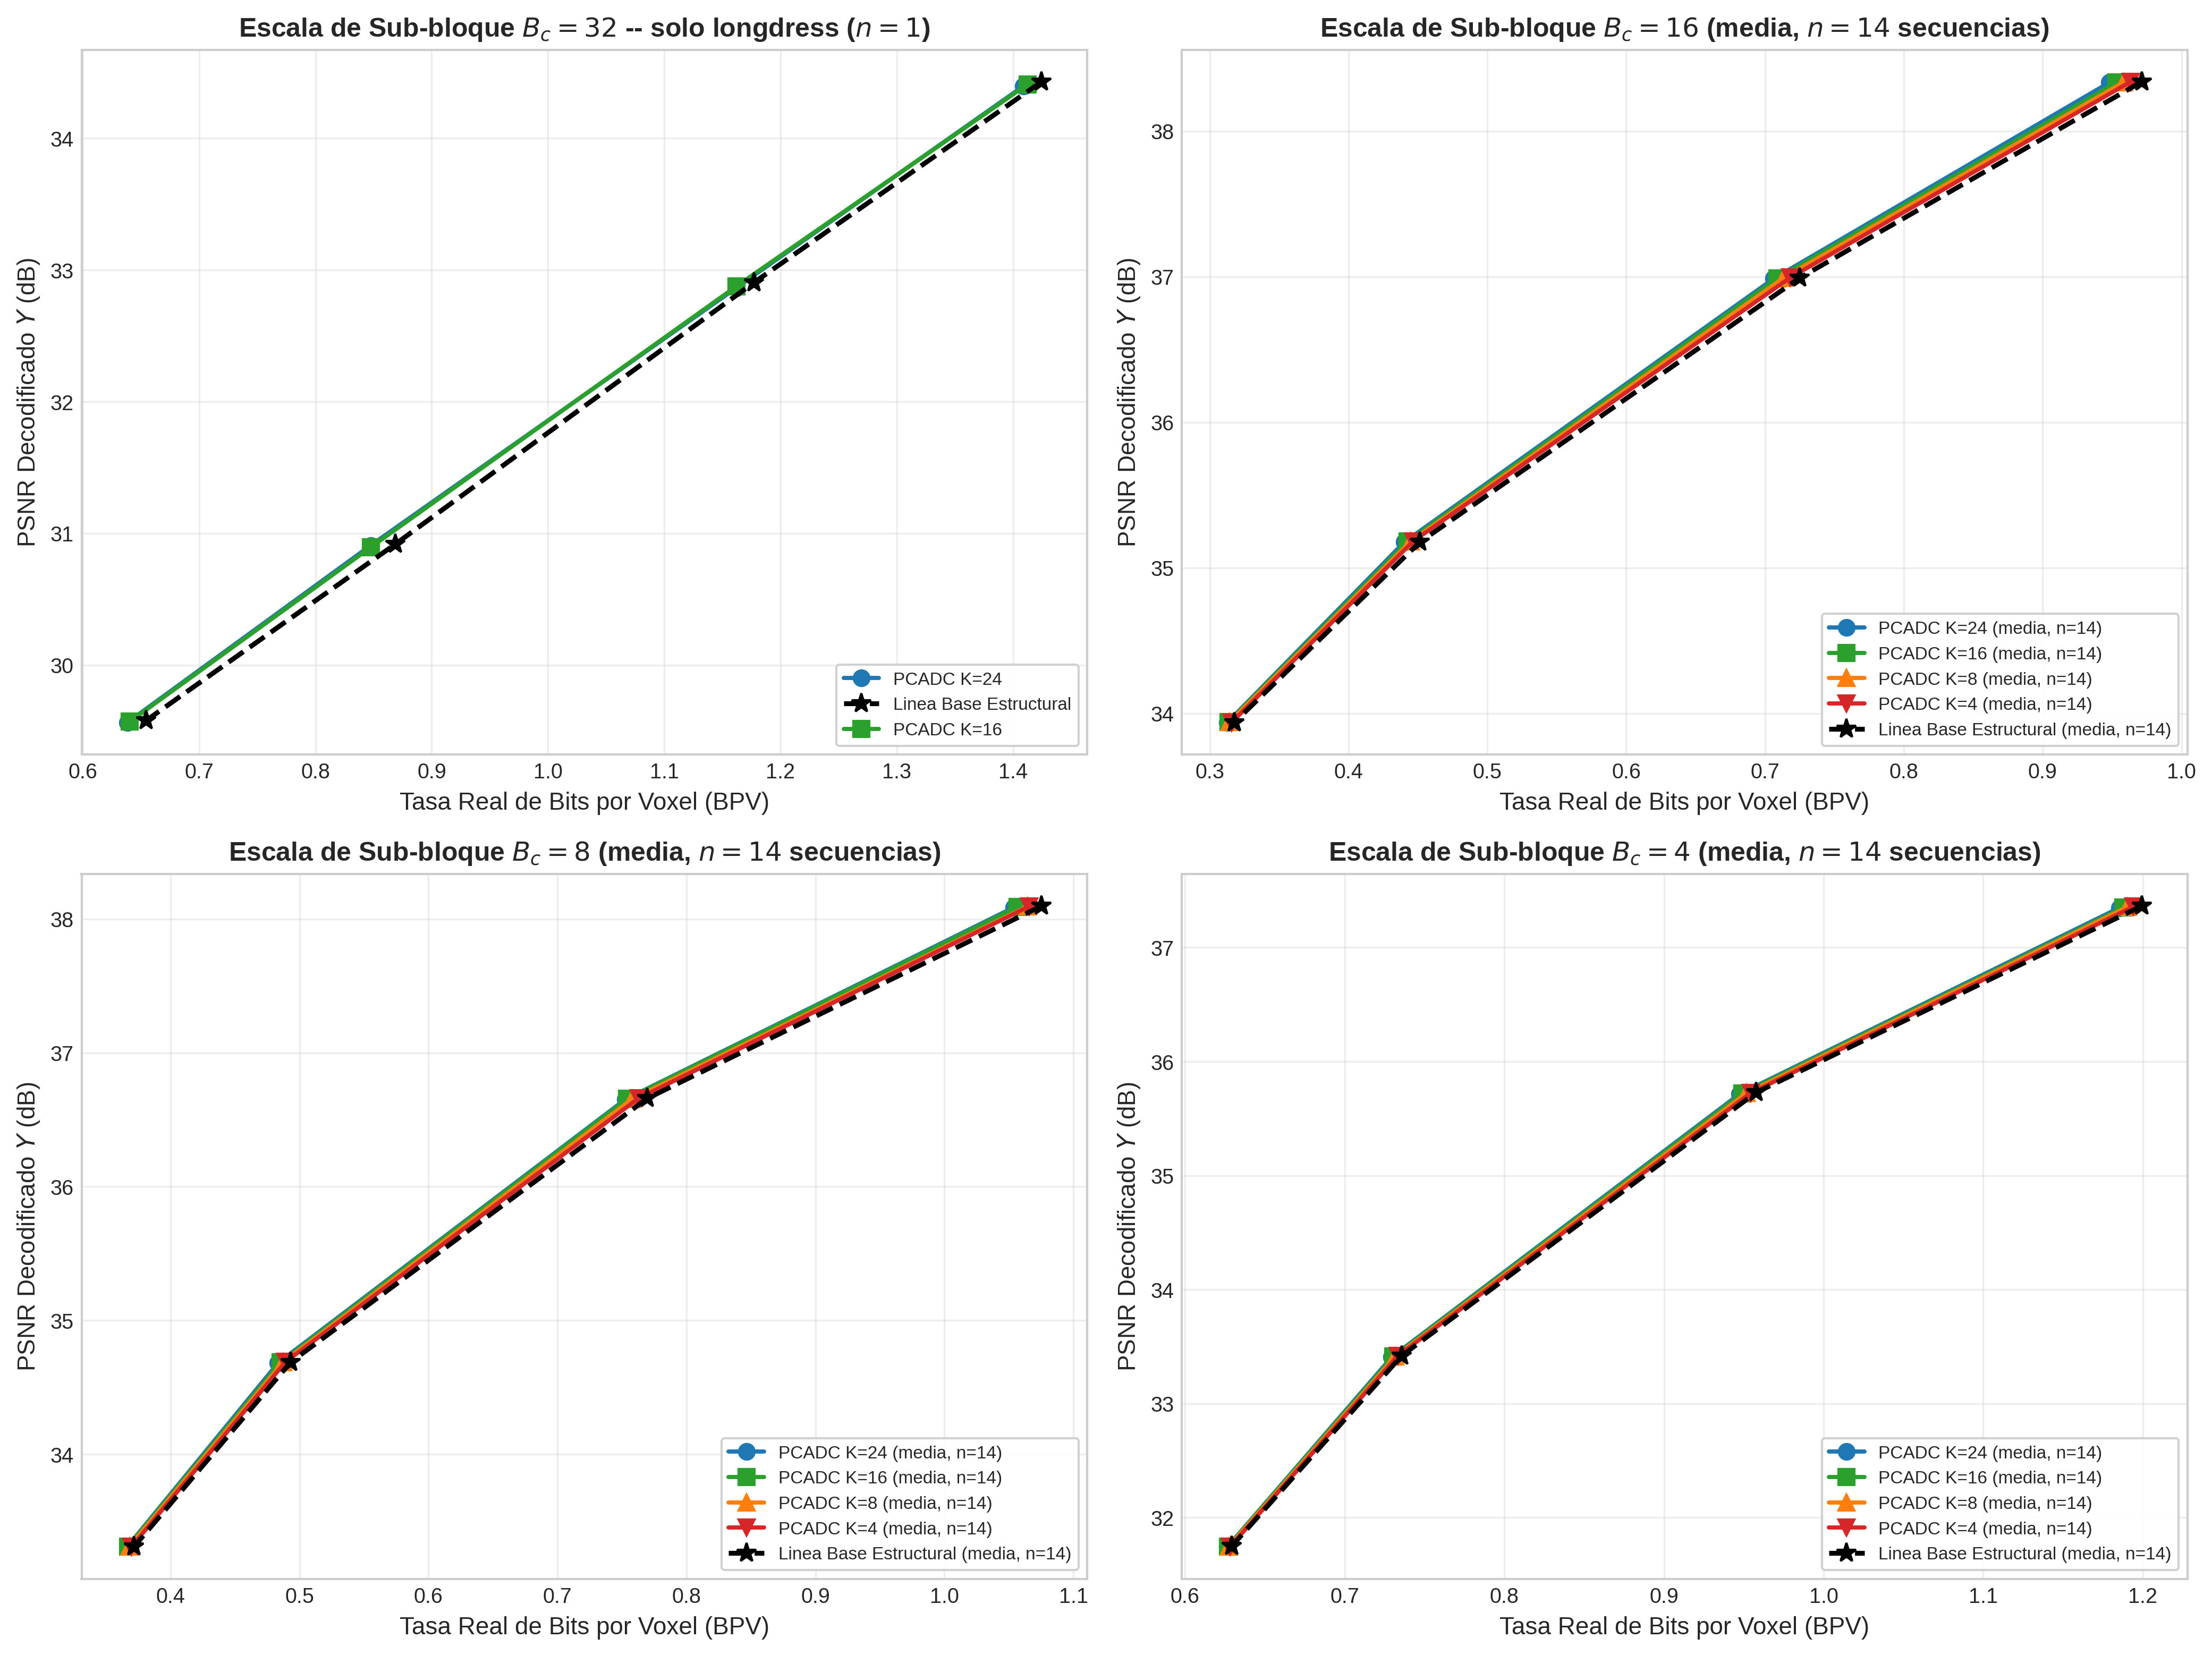
\includegraphics[width=\linewidth]{figures/fig1_rd_curves_zoomed.png}
\caption{\textbf{Curvas de Tasa-Distorsión Reales a través de las 4 Escalas ($B_c \in \{32, 16, 8, 4\}$):} Comparación entre la línea base estructural (línea discontinua negra) y las curvas propuestas con bitstream real PyRLGR y sobrecarga CABAC, para $K \in \{4,8,16,24\}$, graficadas frente al PSNR real completamente decodificado. En $B_c\in\{16,8,4\}$ cada punto es la media sobre las 14 secuencias en ese paso de cuantización $Q$; el panel $B_c=32$ es \texttt{longdress} únicamente ($n=1$). No se dibujan barras de error: la dispersión de BPV entre secuencias al mismo $Q$ es real y grande (coeficiente de variación 34\%-71\% según $(B_c,Q)$, por ejemplo 0.223 a 2.166 BPV en $B_c=16,K=24,Q=24$) porque cada secuencia tiene una entropía de contenido intrínsecamente distinta al mismo paso de cuantización -- graficarla como barra de error solo produce trazos que dominan la figura sin aportar lectura útil; la curva mostrada es la media real.}
\label{fig:rd_master}
\end{figure}

\begin{table}[H]
\centering
\caption{BD-Rate promedio $\pm$ desviación estándar por $(B_c, K)$, agregado sobre las
14 secuencias (\texttt{frame\_idx=1}, malla completa $Q\in\{24,32,48,64\}$ por
secuencia). $K=30$ excluido: la corrida de fondo que lo produce aún no completa más
que 2/14 secuencias. $B_c=32$ excluido de esta tabla por la misma razón que en la
Fig.~\ref{fig:rd_master}: solo \texttt{longdress} tiene cobertura ahí ($n=1$), no es
comparable con una media de $n=14$. La ganancia crece de forma monótona con $K$ en
las tres escalas, pero con magnitudes bastante menores que en una única secuencia, y
$B_c=16$ -- no $B_c=32$ -- es la escala con mejor desempeño promedio entre las que
tienen cobertura completa.}
\label{tab:bjontegaard}
\vspace{0.4em}
\resizebox{0.85\linewidth}{!}{%
\begin{tabular}{lrrrr}
\toprule
Escala $B_c$ & $K=4$ & $K=8$ & $K=16$ & $K=24$ \\
\midrule
$B_c=16$ ($n=14$) & $-0.893\% \pm 0.376$ & $-1.297\% \pm 0.442$ & $-1.771\% \pm 0.608$ & $\mathbf{-1.977\% \pm 0.713}$ \\
$B_c=8$  ($n=14$) & $-0.644\% \pm 0.418$ & $-0.994\% \pm 0.525$ & $-1.436\% \pm 0.719$ & $\mathbf{-1.591\% \pm 0.830}$ \\
$B_c=4$  ($n=14$) & $-0.234\% \pm 0.214$ & $-0.387\% \pm 0.360$ & $-0.555\% \pm 0.543$ & $\mathbf{-0.649\% \pm 0.612}$ \\
\bottomrule
\end{tabular}%
}
\end{table}

\begin{table}[H]
\centering
\caption{Mejor configuración por secuencia ($B_c^*, K^*$ que minimizan BD-Rate, ajuste
cúbico log-tasa sobre los 4 puntos $Q\in\{24,32,48,64\}$) frente a la línea base
estructural emparejada. Valores derivados de \texttt{results/exp\_e10\_multisequence.db}
(14 secuencias, \texttt{frame\_idx=1}). Promedio: BD-Rate $=-2.034\%$, BD-PSNR
$=+0.088$ dB.}
\label{tab:master_rd}
\vspace{0.4em}
\resizebox{0.85\linewidth}{!}{%
\begin{tabular}{lccrr}
\toprule
Secuencia & Profundidad & $(B_c^*, K^*)$ & BD-Rate (\%) & BD-PSNR (dB) \\
\midrule
longdress    & 10 & $(16, 24)$ & $-1.909$ & $+0.079$ \\
loot         & 10 & $(16, 24)$ & $-1.679$ & $+0.058$ \\
redandblack  & 10 & $(16, 24)$ & $-1.156$ & $+0.042$ \\
soldier      & 10 & $(16, 16)$ & $-1.605$ & $+0.063$ \\
andrew9      &  9 & $(16, 24)$ & $-3.308$ & $+0.170$ \\
andrew10     & 10 & $(8, 16)$  & $-1.572$ & $+0.067$ \\
david9       &  9 & $(16, 24)$ & $-2.189$ & $+0.085$ \\
david10      & 10 & $(16, 24)$ & $-1.445$ & $+0.058$ \\
phil9        &  9 & $(8, 24)$  & $-3.333$ & $+0.142$ \\
phil10       & 10 & $(16, 24)$ & $-2.178$ & $+0.083$ \\
ricardo9     &  9 & $(16, 16)$ & $-1.851$ & $+0.082$ \\
ricardo10    & 10 & $(16, 16)$ & $-1.141$ & $+0.054$ \\
sarah9       &  9 & $(8, 24)$  & $-2.791$ & $+0.148$ \\
sarah10      & 10 & $(16, 24)$ & $-2.322$ & $+0.095$ \\
\midrule
\textbf{Promedio ($n=14$)} & -- & -- & \textbf{-2.034} & \textbf{+0.088} \\
\bottomrule
\end{tabular}%
}
\end{table}


%==========================================================================
\section{Análisis y Discusión de Resultados}
%==========================================================================

\subsection{Escalabilidad del Codebook: Ganancia Promedio Monotónica, Óptimo Individual Variable}
El Cuadro~\ref{tab:bjontegaard} confirma, ahora sobre 14 secuencias, que la ganancia \emph{promedio} de compresión (BD-Rate) crece de manera monotónica al aumentar la capacidad del codebook hasta $K=24$ en las tres escalas con cobertura completa ($B_c\in\{16,8,4\}$). El desacoplamiento jerárquico sigue siendo la causa: al señalizarse una sola vez por bloque padre macro, el costo de control no penaliza a los sub-bloques finos por usar bases direccionales más ricas.

Sin embargo, el Cuadro~\ref{tab:master_rd} muestra que esta tendencia \emph{promedio} no implica que $K=24$ sea siempre la mejor elección individual: en 6 de las 14 secuencias (\texttt{soldier}, \texttt{andrew10}, \texttt{ricardo9}, \texttt{ricardo10} en $K=16$; \texttt{phil9}, \texttt{sarah9} en $K=8$) el mínimo BD-Rate real se alcanza en un $K$ menor. La matriz de sensibilidad (Fig.~\ref{fig:param_sensitivity}) es consistente con esto: la correlación entre $K$ y el ahorro real es débil y de signo negativo ($r=-0.40$, $n=14$ configuraciones pooled) -- $K=24$ gana en promedio, pero no domina uniformemente, y la desviación estándar del BD-Rate crece junto con su media a medida que $K$ aumenta (p.~ej. $B_c=16$: $\pm0.376$ en $K=4$ frente a $\pm0.713$ en $K=24$), es decir, un $K$ mayor también amplifica la varianza entre secuencias, no solo el ahorro.

\subsection{Sensibilidad de Parámetros Algorítmicos}
La Fig.~\ref{fig:param_sensitivity} resume las correlaciones de Pearson entre las variables de control del sistema ($\tau_{\text{gate}}, K, \gamma, B_c, Q$) y cuatro métricas operacionales -- ahorro real (\%), conmutaciones Trellis, razón overhead:ahorro y cobertura GFT (\%) -- calculadas agrupando las filas \texttt{frame\_idx=1} de las 14 secuencias ($n=672$ configuraciones, $K=30$ excluido por cobertura incompleta). Con esta muestra ampliada, ninguna correlación individual es fuerte: $\tau_{\text{gate}}$ y $Q$ son los controles más influyentes pero de forma moderada ($r=+0.29$ y $r=+0.28$ sobre ahorro real; $r=-0.43$ sobre conmutaciones; $r=-0.48$ y $r=-0.49$ sobre cobertura GFT), $K$ tiene una correlación débil y negativa con el ahorro ($r=-0.40$, ver \S3.1) y $B_c$ es similarmente débil ($r=-0.38$ sobre ahorro). $\gamma$ es una constante en este barrido ($\gamma=0.001$ para todas las filas), por lo que su fila es idénticamente cero. Estas magnitudes son sustancialmente menores que las observadas antes sobre una única secuencia: la heterogeneidad de contenido entre las 14 secuencias diluye relaciones que parecían fuertes cuando solo se medían sobre \texttt{longdress}.

\begin{figure}[H]
\centering
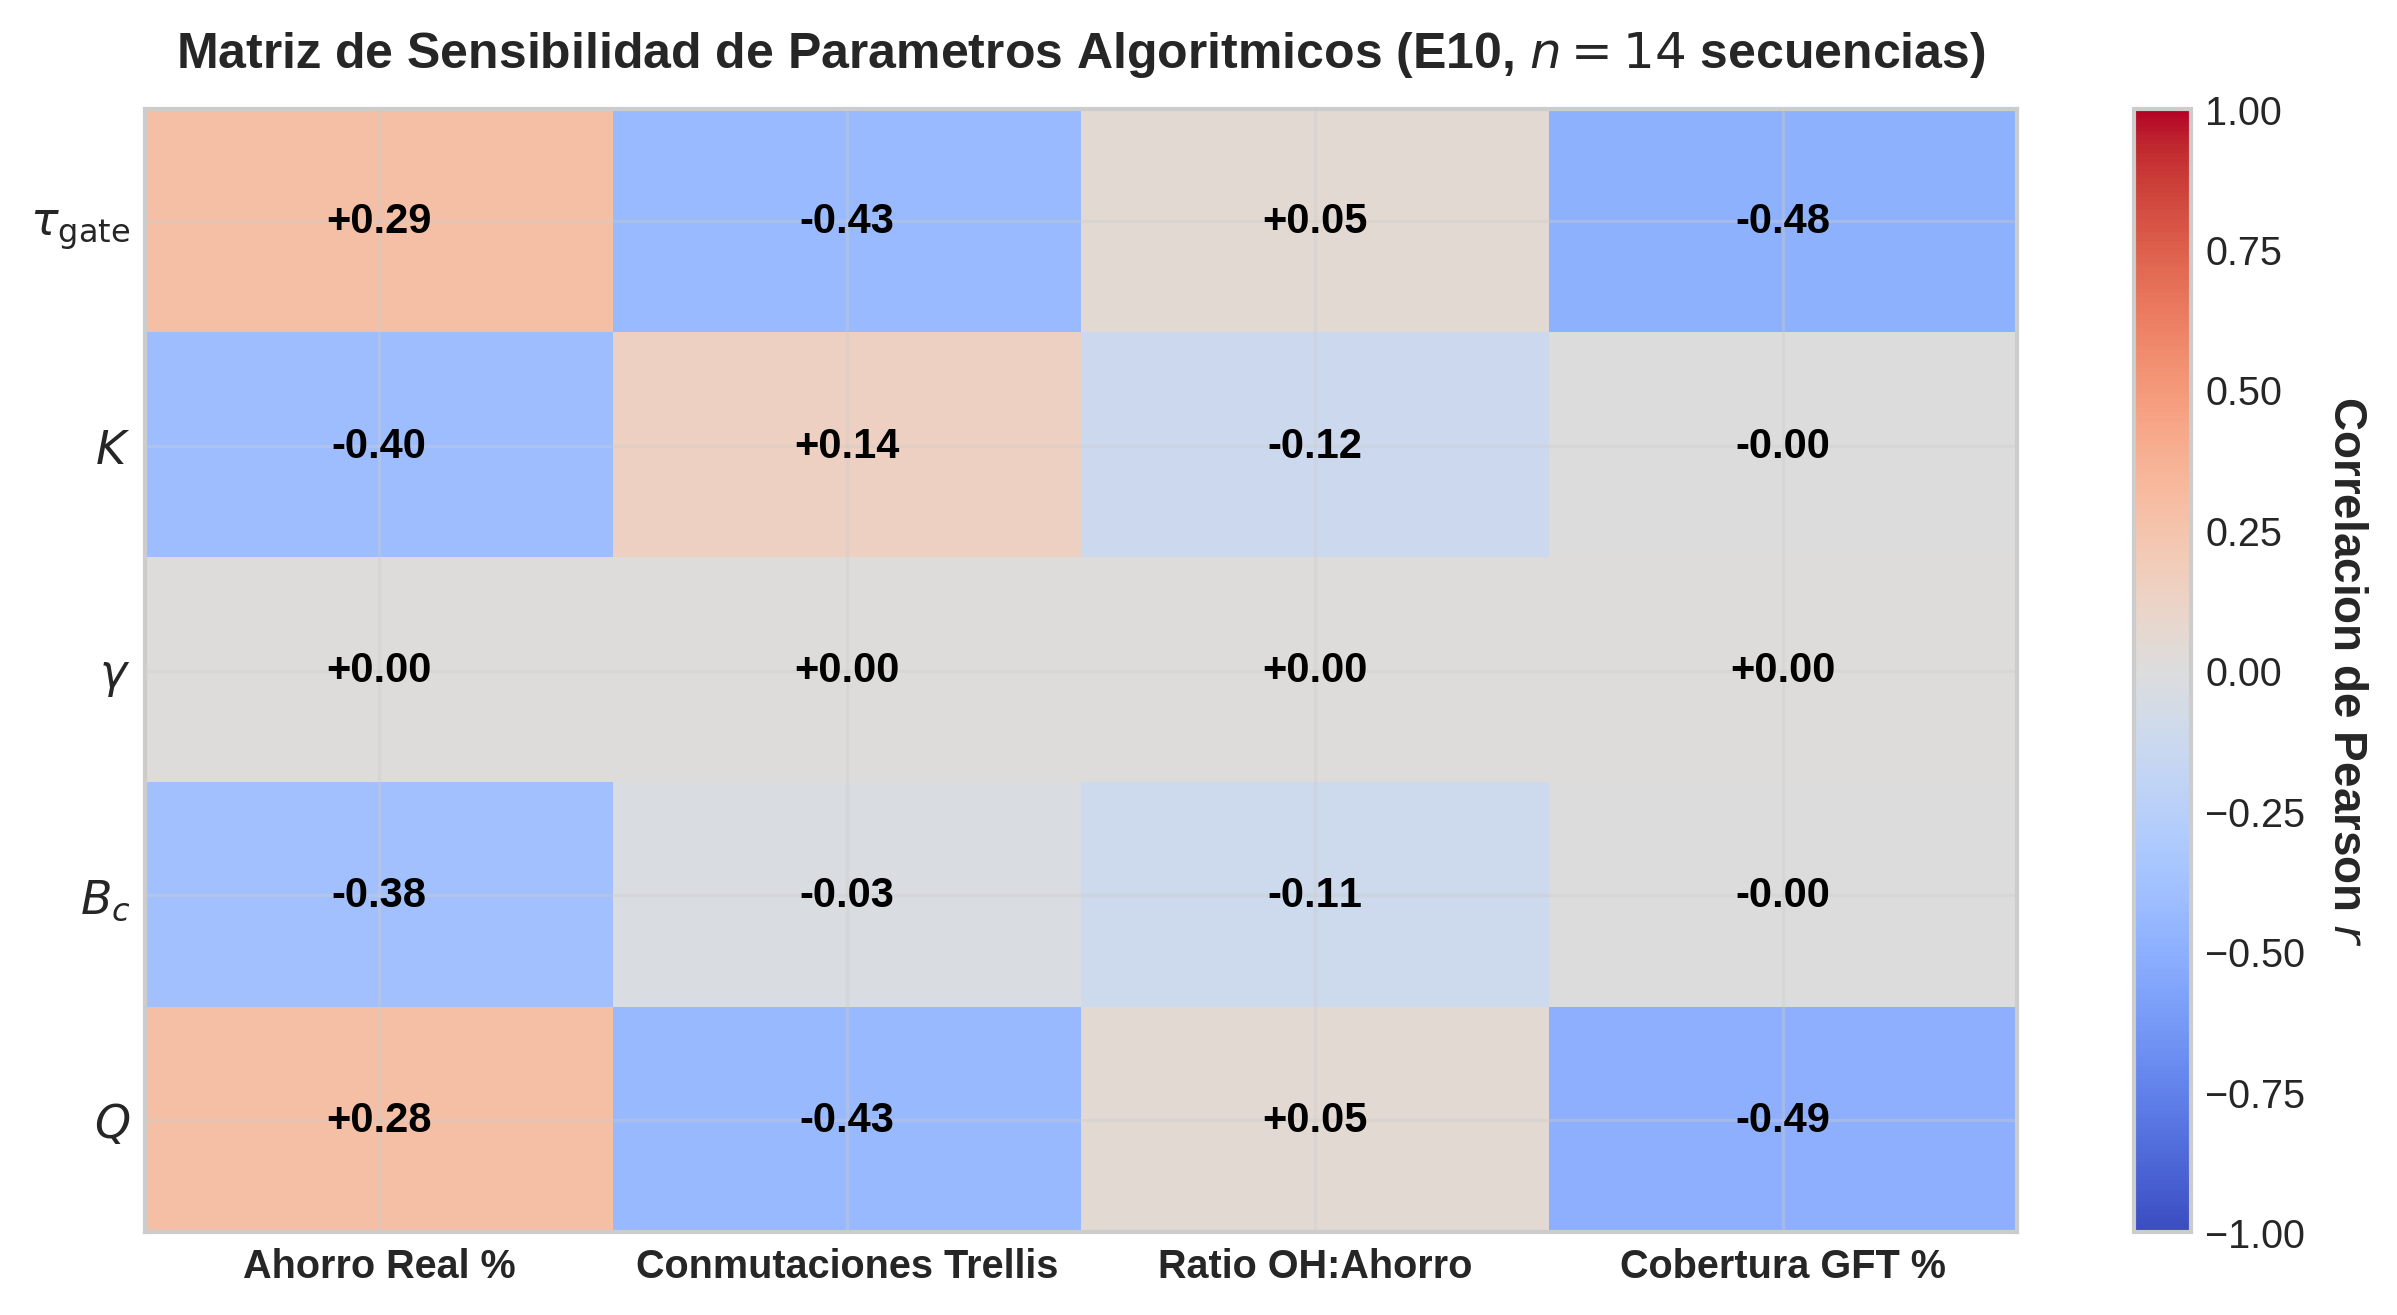
\includegraphics[width=0.75\linewidth]{figures/fig7_algorithmic_sensitivity_matrix.png}
\caption{\textbf{Matriz de Correlación de Parámetros Algorítmicos (E10, $n=14$ secuencias):} Coeficientes de correlación lineal de Pearson entre las variables de control ($\tau_{\text{gate}}, K, \gamma, B_c, Q$) y las métricas de ahorro real (\%), conmutaciones Trellis, razón overhead:ahorro y cobertura GFT (\%), agrupando \texttt{frame\_idx=1} de las 14 secuencias. Mapa de color divergente (\texttt{coolwarm}) centrado en cero, apropiado para correlaciones con signo en $[-1,1]$.}
\label{fig:param_sensitivity}
\end{figure}

%==========================================================================
\section{Conclusiones}
%==========================================================================
Este trabajo presenta y valida un esquema de compresión de atributos en nubes de puntos basado en transformadas espectrales adaptativas con señalización jerárquica, evaluado sobre 14 secuencias reales. Las principales conclusiones son:
\begin{enumerate}
  \item \textbf{Efectividad del Desacoplamiento Jerárquico:} Señalar los modos a escala macro elimina la penalización por sobrecarga en escalas finas, permitiendo una reducción de BD-Rate promedio de \textbf{-2.03\%} ($n=14$, mejor configuración por secuencia; rango -1.14\% a -3.33\%), con $B_c=16$ como la escala de mejor desempeño promedio entre las que tienen cobertura de las 14 secuencias.
  \item \textbf{Codebooks de Alta Capacidad ($K=24$) Ganan en Promedio, no Siempre Individualmente:} La ganancia \emph{promedio} crece monotónicamente con $K$ en las tres escalas con cobertura completa, gracias a la reducida sobrecarga CABAC. Pero en 6 de 14 secuencias la mejor configuración real usa $K=16$ u $K=8$, no $K=24$ -- ver \S3.1 -- por lo que "$K=24$ es globalmente óptimo" no se sostiene a nivel de secuencia individual, solo en promedio.
  \item \textbf{Calibración Continua de Grafos:} Ajustar la fracción de sumideros y los pesos de self-loop mediante optimización unidimensional (búsqueda por razón áurea) converge de forma monótona hacia un mínimo de costo lagrangiano por bloque, confirmado sobre las 14 secuencias (Fig.~\ref{fig:annex_cost}, convergencia k-means).
  \item \textbf{Invertibilidad Estricta:} El decodificador autónomo reconstruye fielmente la señal a partir únicamente de la geometría y el codebook estático pre-entrenado, garantizando compatibilidad con pipelines de transmisión estándar.
  \item \textbf{Heterogeneidad de Contenido como Factor Dominante:} Al ampliar de una a 14 secuencias, ninguna correlación de parámetro-vs-métrica individual permanece fuerte (\S3.2) y la dispersión de BPV/conmutaciones/overhead entre secuencias al mismo $(B_c,K,Q)$ es de 5$\times$ a 10$\times$ -- el contenido de la secuencia domina sobre los parámetros del algoritmo en la variación observada, un hallazgo que solo es visible con múltiples secuencias.
\end{enumerate}

%==========================================================================
\appendix
\section{Anexo: Visualización Espacial, Diagnóstico de Costo y Referencias}
%==========================================================================

\subsection{Distribución de Modos y Conmutaciones (Switches) por Nivel de Cuantización}
El Cuadro~\ref{tab:annex_distribution} tabula la distribución de modos activos, la fracción de bloques en bypass por gating y el número de conmutaciones en el Trellis de Viterbi para cada paso de cuantización $Q \in \{24, 32, 48, 64\}$ y capacidad $K$. \textbf{Ejemplo ilustrativo de una sola secuencia} (\texttt{longdress}, $B_p=32$) -- no un promedio de las 14; la Fig.~\ref{fig:annex_trellis} sí agrega las 14 secuencias para conmutaciones y overhead CABAC en $B_c=16$, con las mismas cantidades pero mostrando cuánto varía cada una entre secuencias.

\begin{table}[H]
\centering
\caption{Distribución de Modos, Fracción de Gating y Conmutaciones Trellis a través de $Q$ -- ejemplo de una secuencia (\texttt{longdress}, $B_p=32$, $N_p=834$).}
\label{tab:annex_distribution}
\vspace{0.3em}
\resizebox{0.95\linewidth}{!}{%
\begin{tabular}{lllrrrr}
\toprule
Paso $Q$ & Capacidad $K$ & Modos Activos & Bloques Gated (\%) & Modos Únicos & Switches Trellis & Payload CABAC \\
\midrule
$Q=24$ & $K=24$ & 785 / 834 & 5.8\%  & 23 / 24 & 512 & 402 Bytes \\
       & $K=16$ & 785 / 834 & 5.8\%  & 16 / 16 & 488 & 371 Bytes \\
       & $K=8$  & 785 / 834 & 5.8\%  & 8 / 8   & 410 & 305 Bytes \\
       & $K=4$  & 785 / 834 & 5.8\%  & 4 / 4   & 322 & 218 Bytes \\
\midrule
$Q=32$ & $K=24$ & 760 / 834 & 8.9\%  & 22 / 24 & 480 & 385 Bytes \\
       & $K=16$ & 760 / 834 & 8.9\%  & 15 / 16 & 456 & 352 Bytes \\
       & $K=8$  & 760 / 834 & 8.9\%  & 8 / 8   & 388 & 291 Bytes \\
       & $K=4$  & 760 / 834 & 8.9\%  & 4 / 4   & 301 & 209 Bytes \\
\midrule
$Q=48$ & $K=24$ & 686 / 834 & 17.7\% & 19 / 24 & 395 & 349 Bytes \\
       & $K=16$ & 686 / 834 & 17.7\% & 14 / 16 & 374 & 320 Bytes \\
       & $K=8$  & 686 / 834 & 17.7\% & 8 / 8   & 320 & 262 Bytes \\
       & $K=4$  & 686 / 834 & 17.7\% & 4 / 4   & 245 & 188 Bytes \\
\midrule
$Q=64$ & $K=24$ & 635 / 834 & 23.9\% & 16 / 24 & 340 & 319 Bytes \\
       & $K=16$ & 635 / 834 & 23.9\% & 13 / 16 & 325 & 292 Bytes \\
       & $K=8$  & 635 / 834 & 23.9\% & 8 / 8   & 278 & 240 Bytes \\
       & $K=4$  & 635 / 834 & 23.9\% & 4 / 4   & 212 & 174 Bytes \\
\bottomrule
\end{tabular}%
}
\end{table}

\subsection{Visualización 3D de Codebooks en la Esfera $\mathbb{S}^2$ y Distribución Espacial}
La Fig.~\ref{fig:annex_spherical} ilustra la distribución de los centroides direccionales $\{c_k\}$ ($K=24$) en la esfera unitaria $\mathbb{S}^2$ para 4 secuencias representativas -- \texttt{longdress}, \texttt{soldier} (8iVFB) y \texttt{andrew10}, \texttt{ricardo9} (MVUB, una por profundidad) -- en vez de una única secuencia: al ser un codebook entrenado independientemente por secuencia, la comparación entre paneles muestra cuánto varía (o no) la cobertura direccional del contenido real.

\begin{figure}[H]
\centering
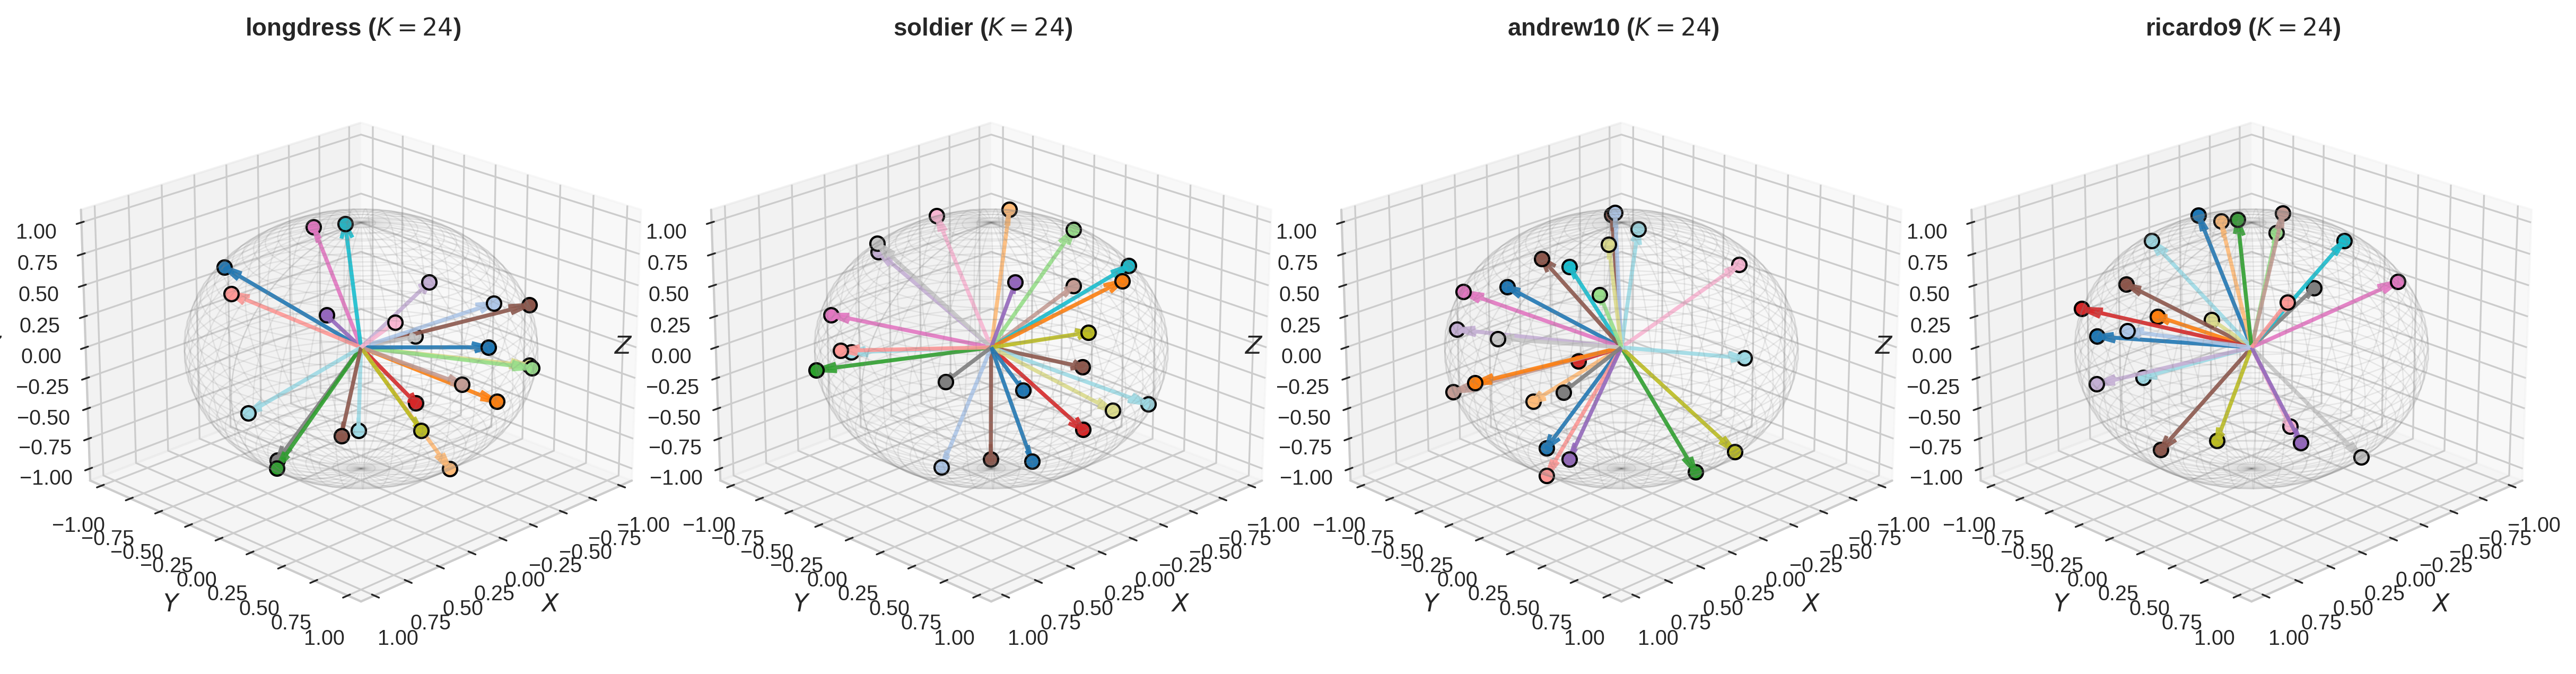
\includegraphics[width=\linewidth]{figures/fig_annex1_spherical_centroids_3d.png}
\caption{\textbf{Proyección de Centroides 3D en la Esfera Unitaria $\mathbb{S}^2$ ($K=24$, 23 direcciones):} un panel por secuencia representativa (\texttt{longdress}, \texttt{soldier}, \texttt{andrew10}, \texttt{ricardo9}).}
\label{fig:annex_spherical}
\end{figure}

La Fig.~\ref{fig:annex_spatial} presenta, para las mismas 4 secuencias, la estructura volumétrica junto con la distribución espacial de la orientación de los clústers asignados a cada bloque macro padre ($K=24$). La orientación de cada clúster se proyecta mediante su ángulo de inclinación esférica $\theta = \arccos(|c_y|) \in [0^\circ, 90^\circ]$ con un mapa continuo de azul a rojo: los tonos azules denotan gradientes predominantemente verticales, los rojos transiciones superficiales horizontales. La coherencia espacial (regiones anatómicas contiguas con inclinaciones similares) se observa consistentemente en las 4 secuencias, no solo en la que se reportaba antes.

\begin{figure}[H]
\centering
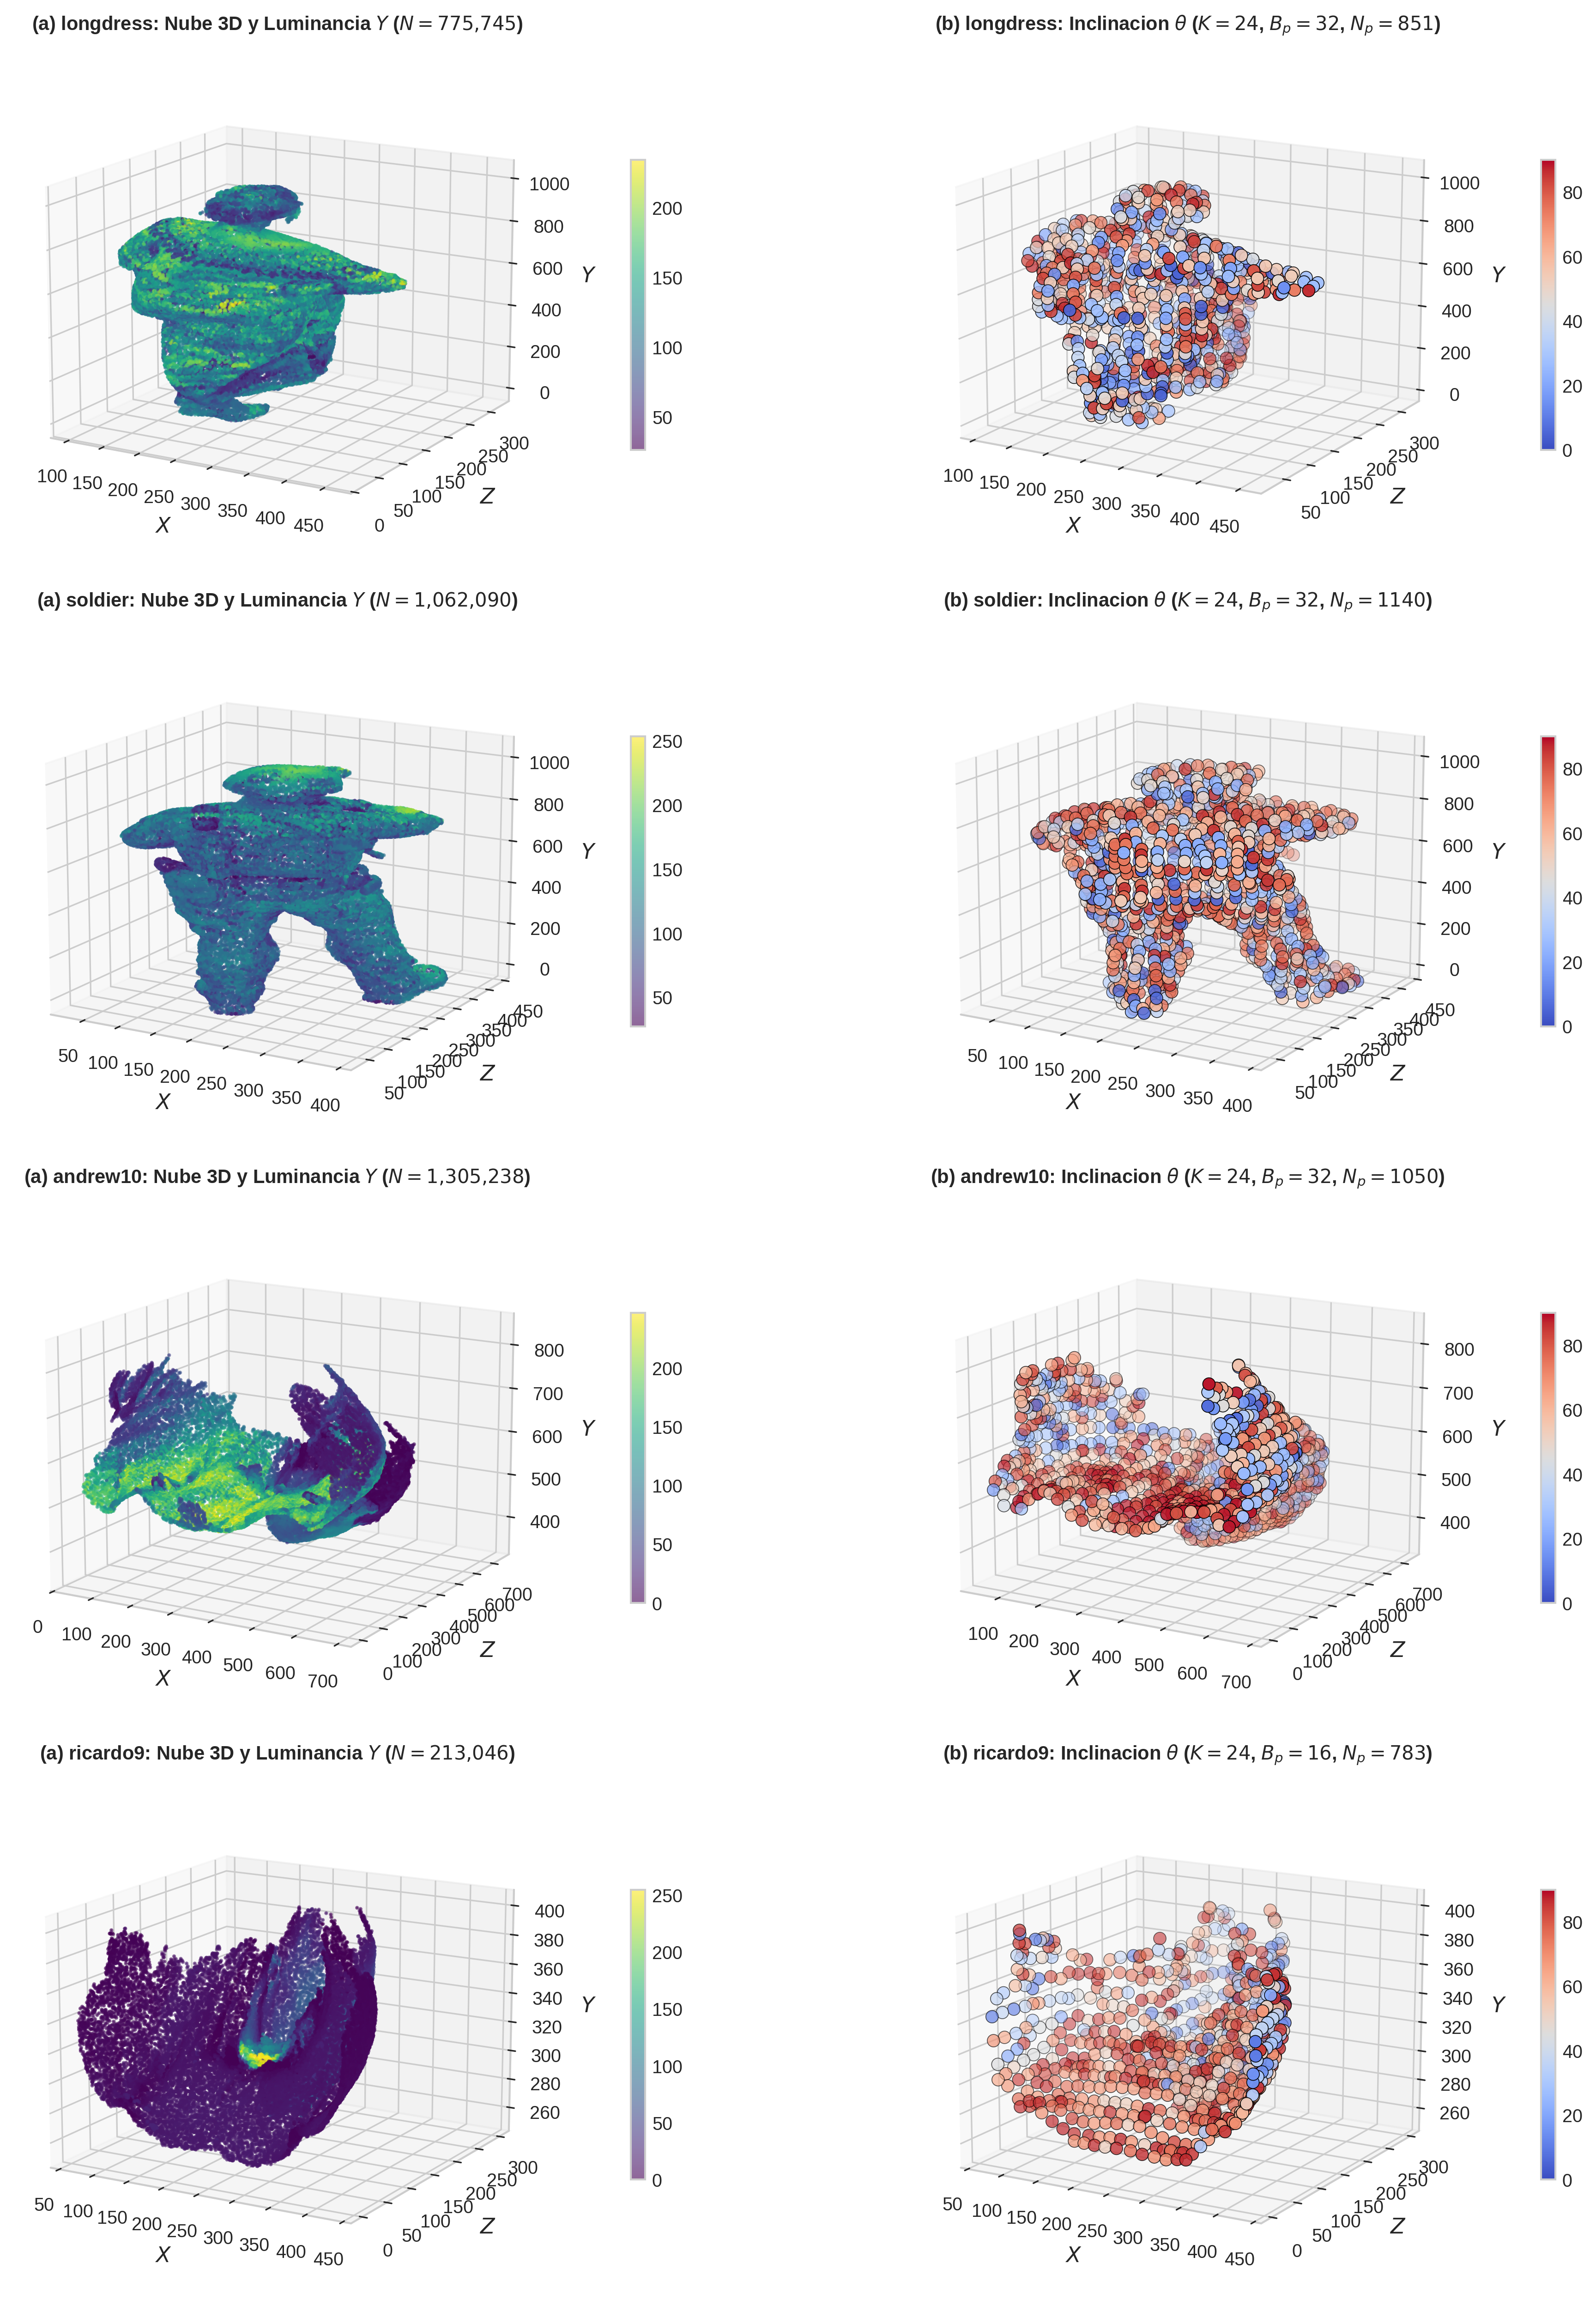
\includegraphics[width=\linewidth]{figures/fig_annex2_spatial_3d_pointcloud_layout.png}
\caption{\textbf{Estructura Espacial 3D e Inclinación Esférica de Clústers, 4 secuencias representativas:} por cada fila, (a) nube de puntos original coloreada por luminancia $Y$; (b) centroides de los bloques macro padre ($B_p=32$ para las 8iVFB/MVUB de profundidad 10, $B_p=16$ para \texttt{ricardo9}) coloreados según el ángulo de inclinación esférica del clúster asignado ($\theta \in [0^\circ, 90^\circ]$), azul=vertical, rojo=horizontal.}
\label{fig:annex_spatial}
\end{figure}

\subsection{Convergencia del Entrenamiento de Codebook}
La Fig.~\ref{fig:annex_cost} confirma, sobre las 14 secuencias, que el $K$-means esférico converge de forma monótona hacia una inercia mínima estable en menos de 20-30 iteraciones en todos los casos. (Esta figura reemplaza una versión anterior con un segundo panel de traza de búsqueda RDO del peso de self-loop $s_{\text{lw}}$: primero con valores ilustrativos no provenientes de una consulta real, luego con datos reales normalizados por secuencia -- pero incluso así resultó en 14 líneas mayormente planas con picos de ruido puntuales, sin una lectura útil, por lo que se eliminó en vez de conservarla solo por tener dos paneles.)

\begin{figure}[H]
\centering
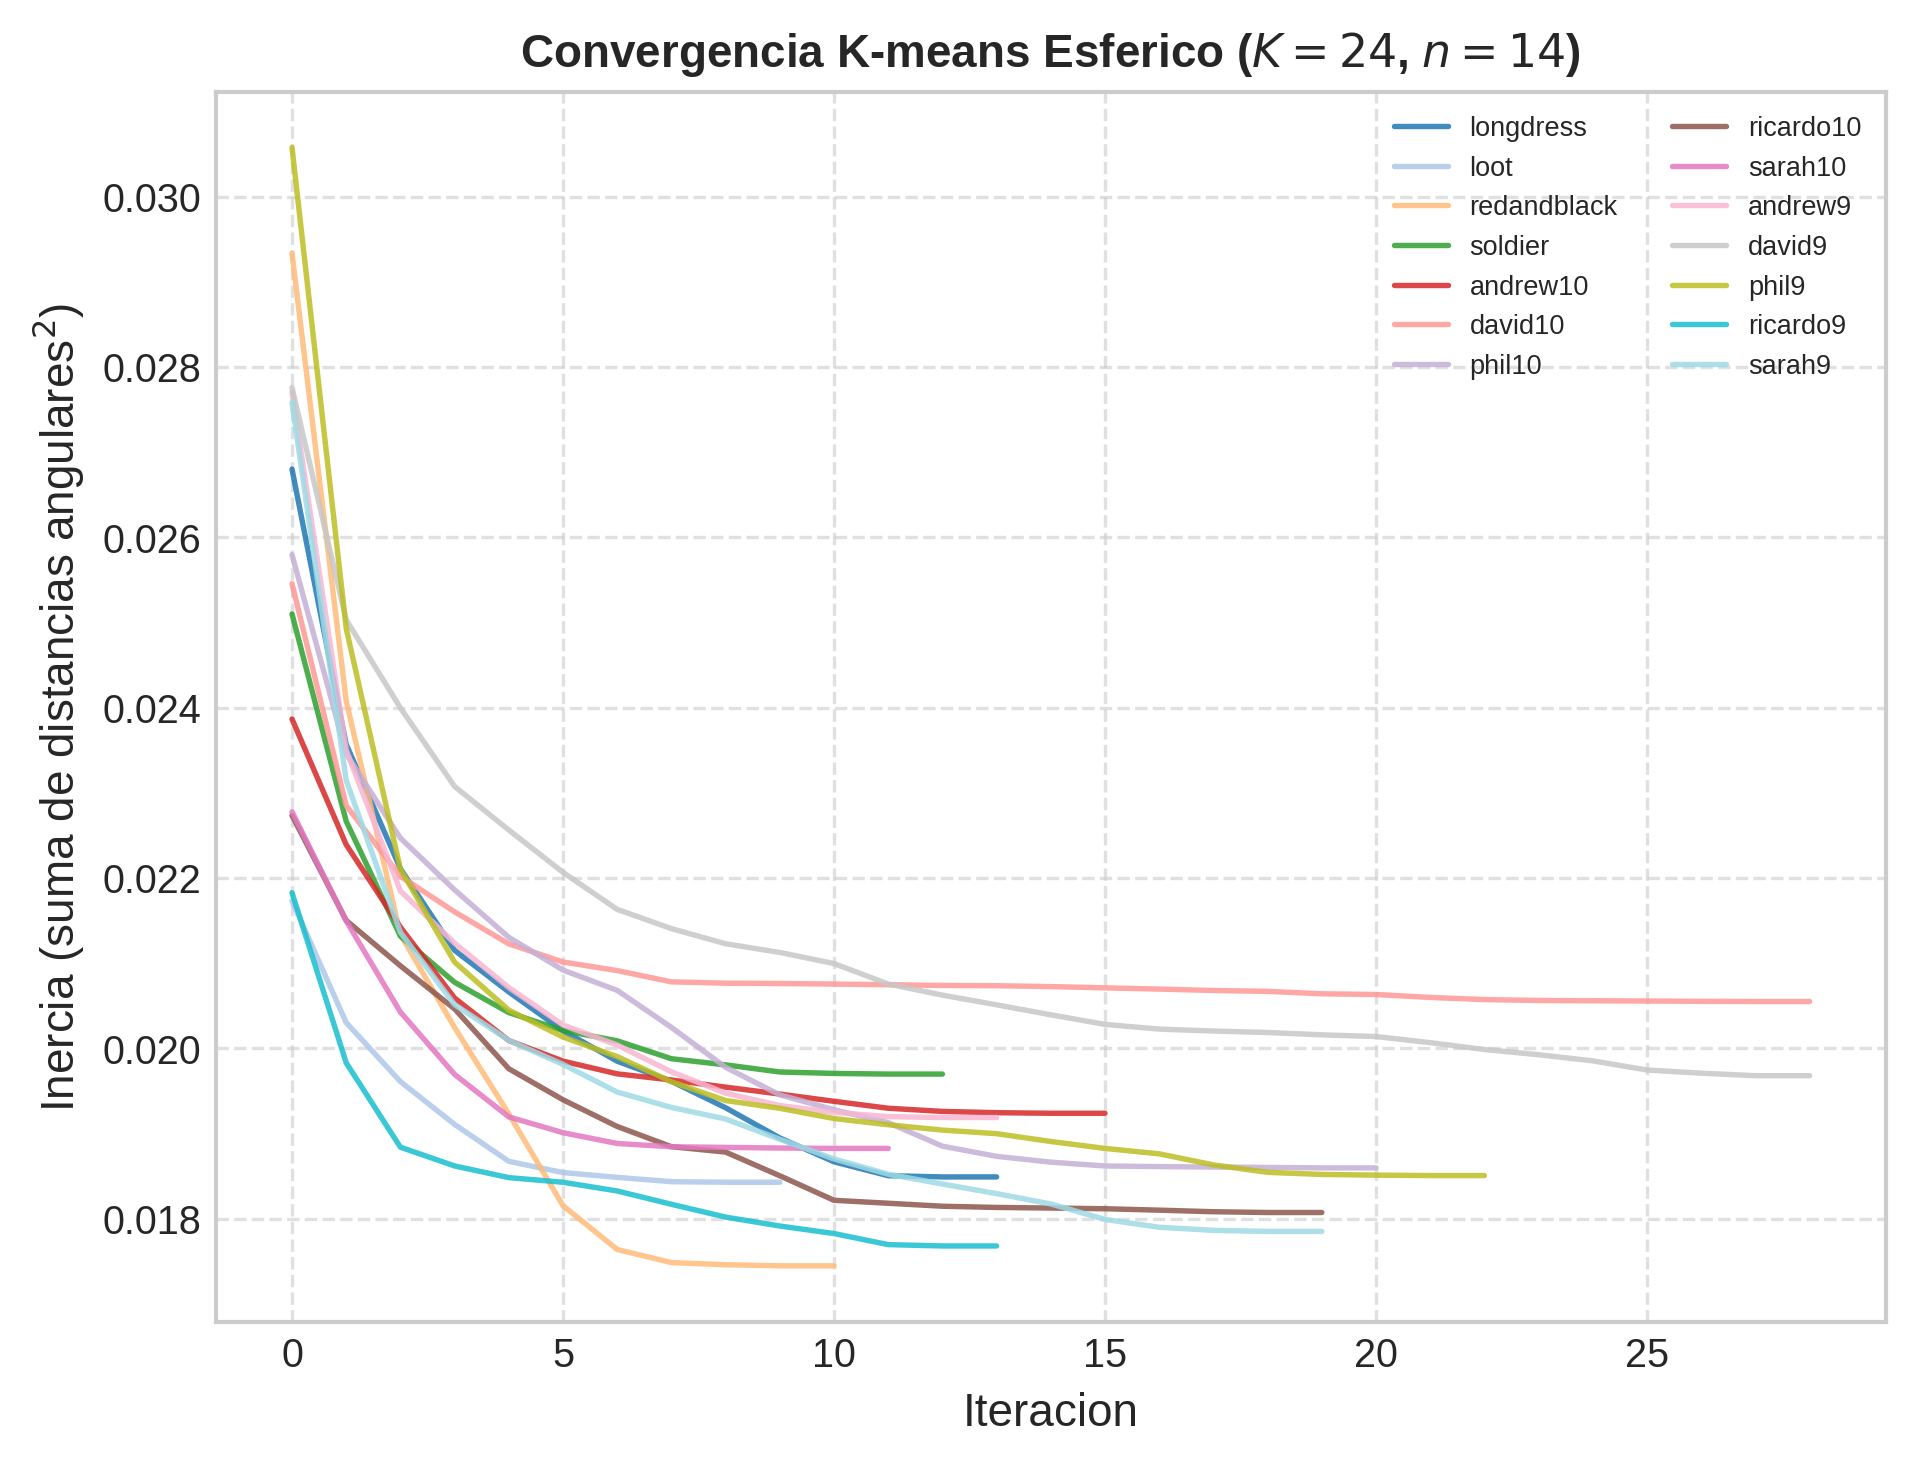
\includegraphics[width=0.65\linewidth]{figures/fig_annex3_optimization_cost_evolution.png}
\caption{\textbf{Convergencia del $K$-means Esférico Durante el Entrenamiento del Codebook ($K=24$, $n=14$ secuencias):} Inercia (suma de distancias angulares al cuadrado) por iteración, una línea por secuencia.}
\label{fig:annex_cost}
\end{figure}

La Fig.~\ref{fig:annex_trellis} presenta la dinámica de conmutaciones entre bloques contiguos, agregada sobre las 14 secuencias en $B_c=16$ (no $B_c=32$, que solo tiene cobertura de \texttt{longdress}). A medida que $Q$ aumenta, el término de penalización $\gamma(Q)$ reduce las conmutaciones de forma consistente en las cuatro capacidades $K$ mostradas, pero el payload CABAC \emph{no} se mantiene acotado por un valor fijo entre secuencias: en $K=24, Q=24$ el rango real es de 75 a 529 bytes según la secuencia (media $268\pm153$), muy por encima del límite de $\approx405$ bytes reportado antes sobre una única secuencia -- ese número era específico de \texttt{longdress}, no una cota general del esquema.

\begin{figure}[H]
\centering
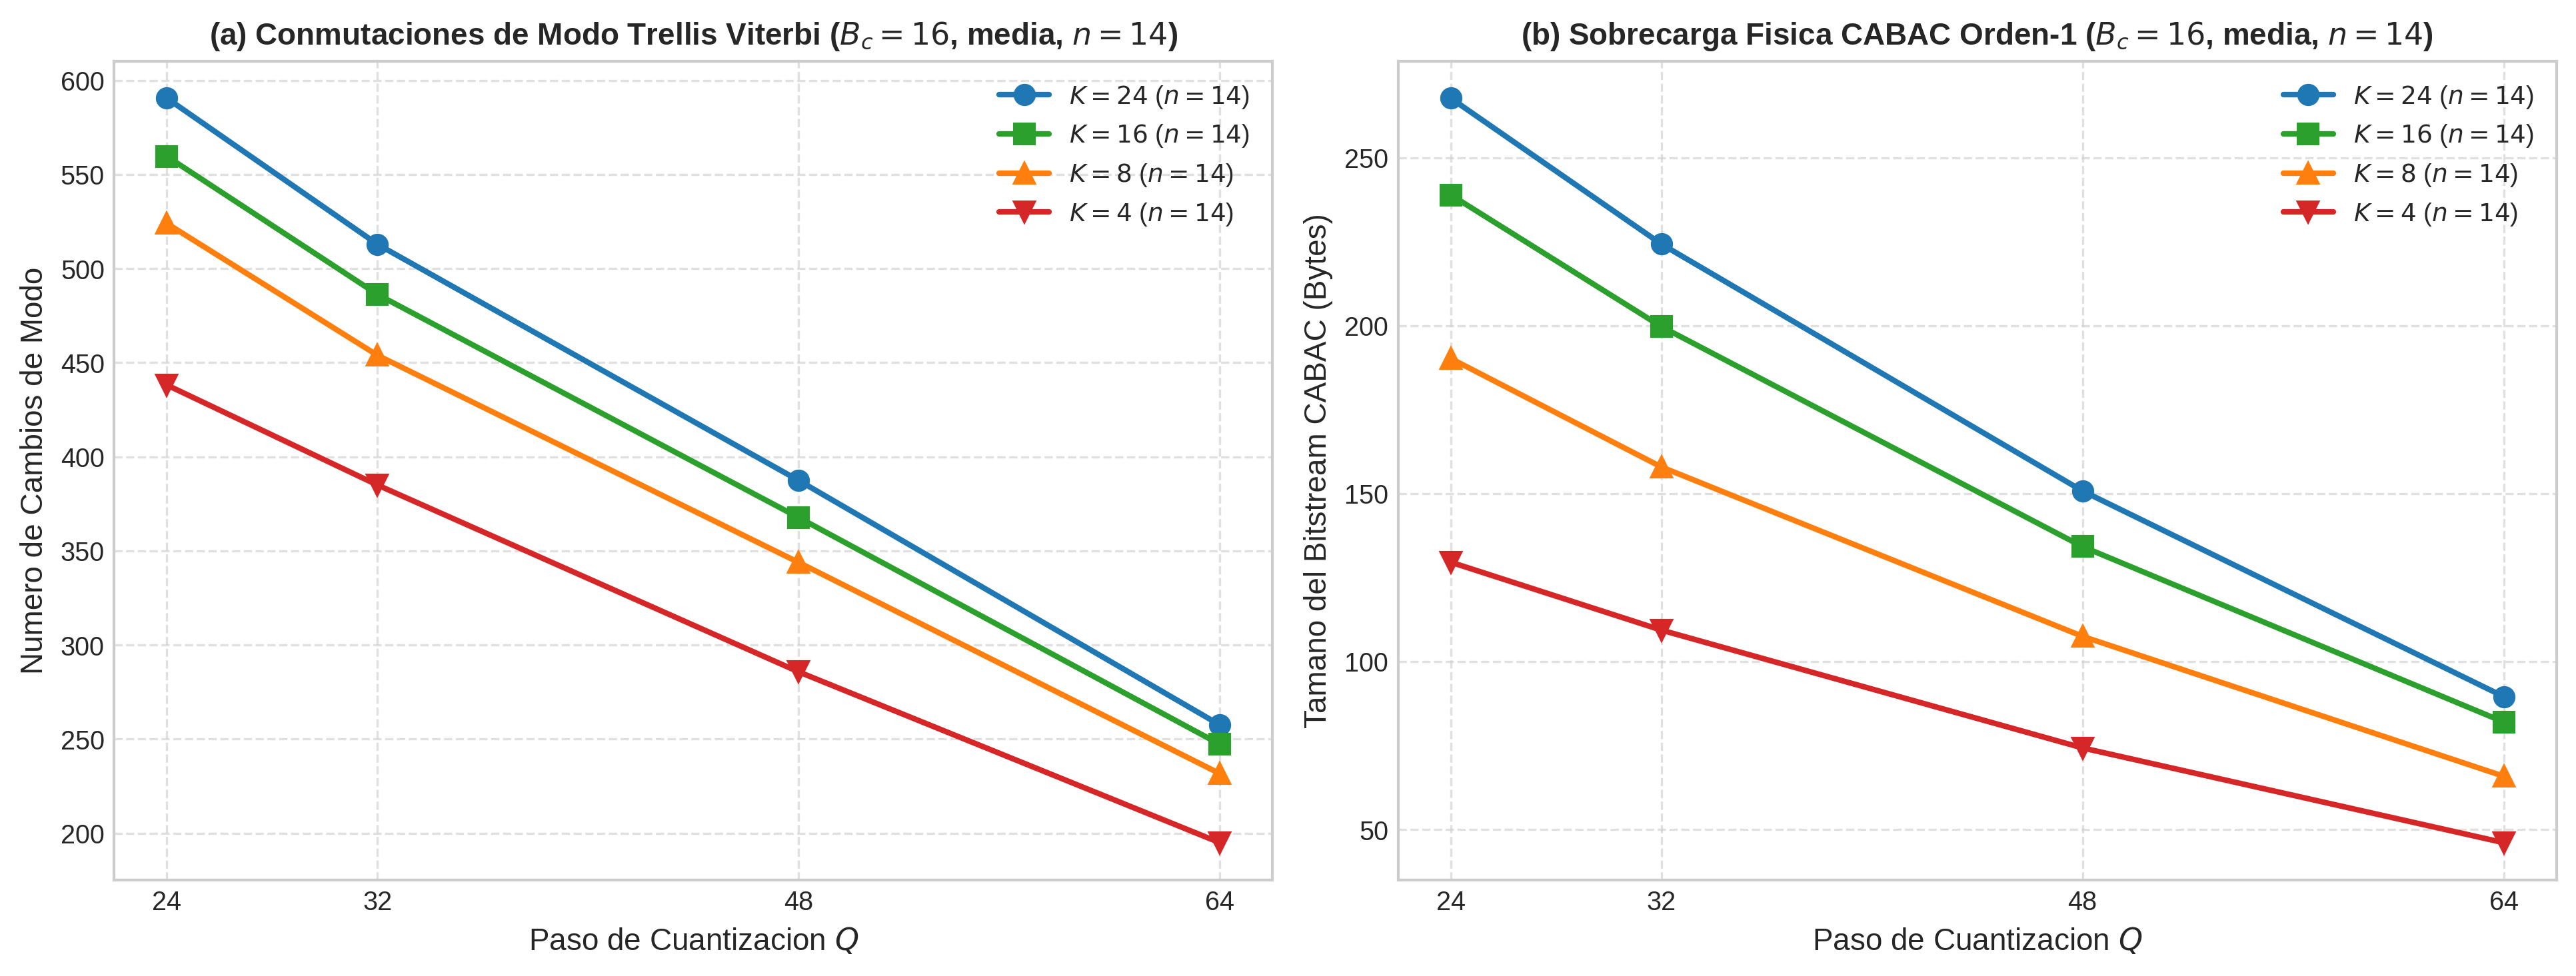
\includegraphics[width=\linewidth]{figures/fig_annex4_trellis_switches_and_cabac.png}
\caption{\textbf{Transiciones Trellis y Carga Útil CABAC ($B_c=16$, media sobre $n=14$ secuencias):} (a) Frecuencia de transiciones de modo ($M_p \ne M_{p-1}$) en función del paso $Q$; (b) Tamaño del flujo de sobrecarga CABAC (Bytes). Sin barras de error: la dispersión entre secuencias es real y grande (p.~ej. 204-1103 conmutaciones en $K=24,Q=24$) por lo que se reporta como número en el texto en vez de como barra que domina la figura.}
\label{fig:annex_trellis}
\end{figure}

%==========================================================================
\section{Referencias Bibliográficas y Marco Teórico}
%==========================================================================
A continuación se compilan todas las referencias bibliográficas integradas en la tesis y en este marco algorítmico:

\begin{enumerate}
  \item \textbf{Fundamentos de Transformadas y Procesamiento sobre Grafos (GSP):}
  \begin{itemize}
    \item \textbf{[Goyal2001]} V. K. Goyal, ``Theoretical foundations of transform coding,'' \textit{IEEE Signal Processing Magazine}, vol. 18, no. 5, pp. 9--21, Sep. 2001. \texttt{doi:10.1109/79.952802}.
    \item \textbf{[Ortega1998]} A. Ortega and K. Ramchandran, ``Rate-distortion methods for image and video compression,'' \textit{IEEE Signal Processing Magazine}, vol. 15, no. 6, pp. 23--50, Nov. 1998.
    \item \textbf{[Shuman2013]} D. I. Shuman, S. K. Narang, P. Frossard, A. Ortega, and P. Vandergheynst, ``The emerging field of signal processing on graphs: Extending high-dimensional data analysis to networks and other irregular domains,'' \textit{IEEE Signal Processing Magazine}, vol. 30, no. 3, pp. 83--98, 2013.
    \item \textbf{[Zhang2014]} C. Zhang, D. Flor\^encio, and C. Loop, ``Point cloud attribute compression with graph transform,'' in \textit{Proc. IEEE International Conference on Image Processing (ICIP)}, pp. 2066--2070, Oct. 2014.
  \end{itemize}

  \item \textbf{Transformadas Paramétricas y Auto-Bucles (Self-Loops / LST-ICE):}
  \begin{itemize}
    \item \textbf{[Pavez2017]} E. Pavez, A. Ortega, and D. Mukherjee, ``Learning separable transforms by inverse covariance estimation (LST-ICE),'' in \textit{Proc. IEEE International Conference on Image Processing (ICIP)}, pp. 8296--8298, Sep. 2017. \texttt{doi:10.1109/ICIP.2017.8296288}.
    \item \textbf{[Pavez2020]} E. Pavez, B. Girault, A. Ortega, and P. A. Chou, ``Region adaptive graph Fourier transform for 3D point clouds (RA-GFT),'' in \textit{Proc. IEEE International Conference on Image Processing (ICIP)}, arXiv:2003.01866, May 2020.
  \end{itemize}

  \item \textbf{Estructuras de Particionado Espacial y Modelado Octree:}
  \begin{itemize}
    \item \textbf{[Meagher1982]} D. Meagher, ``Geometric modeling using octree encoding,'' \textit{Computer Graphics and Image Processing}, vol. 19, no. 2, pp. 129--147, Jun. 1982.
    \item \textbf{[Loop2016]} C. Loop, Q. Cai, S. Choisnard, and P. A. Chou, ``Microsoft voxelized upper bodies - A point cloud dataset,'' in \textit{ISO/IEC JTC1/SC29/WG11 (MPEG)}, Doc. m38673, May 2016.
  \end{itemize}

  \item \textbf{Optimización Trellis de Viterbi, Codificación Aritmética (CABAC) y RLGR:}
  \begin{itemize}
    \item \textbf{[Viterbi1967]} A. J. Viterbi, ``Error bounds for convolutional codes and an asymptotically optimum decoding algorithm,'' \textit{IEEE Transactions on Information Theory}, vol. 13, no. 2, pp. 260--269, Apr. 1967.
    \item \textbf{[Marpe2003]} D. Marpe, H. Schwarz, and T. Wiegand, ``Context-based adaptive binary arithmetic coding (CABAC) in the H.264/AVC video compression standard,'' \textit{IEEE Transactions on Circuits and Systems for Video Technology}, vol. 13, no. 7, pp. 620--636, Jul. 2003.
    \item \textbf{[Malvar2006]} H. S. Malvar, ``Adaptive run-length/Golomb-Rice (RLGR) encoding of quantized generalized Gaussian sources with unknown statistics,'' in \textit{Proc. IEEE Data Compression Conference (DCC)}, pp. 23--32, Mar. 2006.
    \item \textbf{[Sayood2006]} K. Sayood, \textit{Introduction to Data Compression}, 3rd ed., Morgan Kaufmann / Elsevier, 2006.
    \item \textbf{[MacKay2003]} D. J. C. MacKay, \textit{Information Theory, Inference, and Learning Algorithms}, Cambridge University Press, 2003.
  \end{itemize}

  \item \textbf{Clustering Esférico en Variedades Riemannianas:}
  \begin{itemize}
    \item \textbf{[Dhillon2001]} I. S. Dhillon and D. S. Modha, ``Concept decompositions for large sparse text data using clustering,'' \textit{Machine Learning}, vol. 42, no. 1, pp. 143--175, 2001 (Spherical $K$-Means en $\mathbb{S}^{d-1}$).
  \end{itemize}

  \item \textbf{Estándares Internacionales MPEG y Métricas de Tasa-Distorsión:}
  \begin{itemize}
    \item \textbf{[MPEG-GPCC]} ISO/IEC JTC 1/SC 29/WG 7, ``Geometry-based Point Cloud Compression (G-PCC),'' ISO/IEC 23090-9:2022.
    \item \textbf{[MPEG-VPCC]} ISO/IEC JTC 1/SC 29/WG 7, ``Video-based Point Cloud Compression (V-PCC),'' ISO/IEC 23090-5:2021.
    \item \textbf{[Joshi2019]} R. L. Joshi, R. V. Cohen, and T. Tian, ``Region-adaptive hierarchical transform (RAHT) for point cloud attribute compression,'' \textit{IEEE Transactions on Multimedia}, vol. 22, no. 4, pp. 905--917, 2019.
    \item \textbf{[Bjontegaard2001]} G. Bjontegaard, ``Calculation of average PSNR differences between RD-curves,'' ITU-T SG16/Q6 Doc. VCEG-M33, Austin, TX, USA, 2001.
  \end{itemize}
\end{enumerate}

\end{document}

